\documentclass[a4paper,11pt]{article}%必须以此为开头,可以在[]内设置栏数,单双面,横竖向
\usepackage{latexsym}%符号字体
\usepackage{makeidx}%制作索引
\makeindex
\usepackage{ifthen}%提供分支语句
\usepackage{ctex}%提供中文支持
\usepackage{graphicx}%用于插入图片
\usepackage{amsmath}%用于数学公式
\usepackage{IEEEtrantools}%用于使用IEEE数学公式排版工具
\usepackage{amsfonts}%用于其他字体的数学符号
\usepackage{amsthm}%提供证明,定理等环境
\usepackage{amssymb}%用于提供各种数学符号
\usepackage{mathrsfs}%用于提供花体字母
\usepackage{verbatim}%使用\verbatiminput{filename}来直接导入文件中的文本内容
\usepackage{layouts}%用于设置页面布局
\usepackage{calc}%允许一些常量参量用算术表达式代替
\usepackage{hyperref}
\usepackage{makecell}%允许表格的单元格内换行
\usepackage{bm}%使用bm来对希腊字母加粗
\usepackage{longtable}
\usepackage{slashed}
\usepackage[hmargin=1.25in,vmargin=1in]{geometry}
\usepackage{adjustbox}%强行让图片置中
\theoremstyle{remark}
\newtheorem*{remark}{注}
\theoremstyle{remark}
\newtheorem*{example}{例}
\theoremstyle{definition}
\newtheorem{theorem}{定理}[section]
\theoremstyle{definition}
\newtheorem*{definition}{定义}
\theoremstyle{definition}
\newtheorem{corollary}{引理}[section]
\newcommand*{\abs}[1]{\lvert #1 \rvert}
%伪代码
\usepackage{algorithm}
\usepackage{algorithmicx}
\usepackage{algpseudocode}
\usepackage{amsmath}
%伪代码
%代码块
\usepackage{ listings}
\usepackage[x11names]{xcolor}
\definecolor{mygreen}{rgb}{0,0.6,0}
\definecolor{mygray}{rgb}{0.5,0.5,0.5}
\definecolor{mymauve}{rgb}{0.58,0,0.82}
\lstset{ %
	backgroundcolor=\color{white},      % choose the background color
	basicstyle=\footnotesize\ttfamily,  % size of fonts used for the code
	columns=fullflexible,
	tabsize=4,
	breaklines=true,               % automatic line breaking only at whitespace
	captionpos=b,                  % sets the caption-position to bottom
	commentstyle=\color{mygreen},  % comment style
	escapeinside={\%*}{*)},        % if you want to add LaTeX within your code
	keywordstyle=\color{blue},     % keyword style
	stringstyle=\color{mymauve}\ttfamily,  % string literal style
	frame=single,
	rulesepcolor=\color{red!20!green!20!blue!20},
	% identifierstyle=\color{red},
	language=c,
}
%代码块
%引用
\usepackage{framed}
\usepackage{quoting}
 \colorlet{shadecolor}{Turquoise1!20}
\newenvironment{shadedquotation}
 {\begin{shaded*}
  \quoting[leftmargin=0pt, vskip=0pt]
 }
 {\endquoting
 \end{shaded*}
}
%引用
%跨页伪代码
\makeatletter
\newenvironment{breakablealgorithm}
  {% \begin{breakablealgorithm}
   \begin{center}
     \refstepcounter{algorithm}% New algorithm
     \hrule height.8pt depth0pt \kern2pt% \@fs@pre for \@fs@ruled
     \renewcommand{\caption}[2][\relax]{% Make a new \caption
       {\raggedright\textbf{\ALG@name~\thealgorithm} ##2\par}%
       \ifx\relax##1\relax % #1 is \relax
         \addcontentsline{loa}{algorithm}{\protect\numberline{\thealgorithm}##2}%
       \else % #1 is not \relax
         \addcontentsline{loa}{algorithm}{\protect\numberline{\thealgorithm}##1}%
       \fi
       \kern2pt\hrule\kern2pt
     }
  }{% \end{breakablealgorithm}
     \kern2pt\hrule\relax% \@fs@post for \@fs@ruled
   \end{center}
  }
\makeatother
%跨页伪代码
\floatname{algorithm}{算法}
\renewcommand{\algorithmicrequire}{\textbf{输入:}}
\renewcommand{\algorithmicensure}{\textbf{输出:}}
\author{范潇}
\title{K-Means算法实验报告}
\date{2023年12月17日}
\begin{document}
\lstset{breaklines}%这条命令可以让LaTeX自动将长的代码行换行排版
		\lstset{extendedchars=false}%这一条命令可以解决代码跨页时,章节标题,页眉等汉字不显
		%示的问题
		\lstset{numbers=left,numberstyle=\tiny,keywordstyle=\color{blue!70},
			commentstyle=\color{red!50!green!50!blue!50},frame=shadowbox,
			rulesepcolor=\color{red!20!green!20!blue!20},escapeinside=``,
			%xleftmargin=-10em,xrightmargin=-23em,
            aboveskip=1em} 
\pagestyle{plain}
\maketitle
\section{实验内容}
在本次实验中,我使用Python语言实现二分K-Means,并使用matplotlib库对聚类结果进行可视化。

实验过程为:
\begin{enumerate}
    \item 选择数据集
    \item 数据集预处理
    \item 实现二分 K-Means 算法
    \item 对算法进行评价
    \item 可视化
\end{enumerate}
\section{函数说明}
在实现该算法的过程中,使用的主要数据结果为DataFrame。数据集的原始数据存储在 data变量中,并且最后一列'origin\_row'存储的是各个行的行标;
经过 t-SNE,降维后的数据存储在 reduced变量中,并且最后两列分别为 'origin\_row'和用于存储所属类簇信息的'color'列。
\subsection{求类簇SSE}
\begin{lstlisting}[language={Python},keywordstyle=\color{blue!70},commentstyle=\color{red!50!green!50!blue!50},frame=shadowbox,
    rulesepcolor=\color{red!20!green!20!blue!20}]
def get_sse(df):
    sse = ((df.iloc[:, :-1] - df.iloc[:, :-1].mean(axis=0, numeric_only=True)) ** 2).sum().sum()
    # 减去平均值后求平方,然后对矩阵中的所有元素进行求和
    return sse
\end{lstlisting}
\subsection{类簇二分}
\begin{lstlisting}[language={Python},keywordstyle=\color{blue!70},commentstyle=\color{red!50!green!50!blue!50},frame=shadowbox,
    rulesepcolor=\color{red!20!green!20!blue!20}]
def split(df):
    # 随机挑选两个初始点
    init1 = random.randint(0, df.shape[0] - 1)
    init2 = random.randint(0, df.shape[0] - 1)
    while init2 == init1:
        init2 = random.randint(0, df.shape[0] - 1)
    df1 = df[((df - df.iloc[init1, :-1]) ** 2).sum(axis=1) <= ((df - df.iloc[init2, :-1]) ** 2).sum(axis=1)]
    df2 = df[((df - df.iloc[init2, :-1]) ** 2).sum(axis=1) < ((df - df.iloc[init1, :-1]) ** 2).sum(axis=1)]
    # 返回分裂所得的两个数据表,以及它们的和方差之和
    return df1, df2, get_sse(df1) + get_sse(df2)
\end{lstlisting}
本函数利用DataFrame的布尔过滤功能来实现分裂
\subsection{求轮廓系数}
\begin{lstlisting}[language={Python},keywordstyle=\color{blue!70},commentstyle=\color{red!50!green!50!blue!50},frame=shadowbox,
    rulesepcolor=\color{red!20!green!20!blue!20}]
def make_silhouette(clusters):
    # 求各类簇的中心
    center = []
    for cluster in clusters:
        center.append(cluster.iloc[:, :-1].mean())
    center = pd.DataFrame(center)
    # 用于存储由各类簇中的数据的轮廓系数所组成的list
    alphas = []
    for i, cluster in enumerate(clusters):
        alpha = []
        for j, data in enumerate(cluster.values):
            # 求到簇内其他数据的平均距离
            a = (((cluster.iloc[:, :-1] - data[:-1]) ** 2).sum(axis=1) ** 0.5).mean(axis=0)
            # 求最近的其他类簇中心
            nearest = (((center - data[:-1]) ** 2).sum(axis=1).drop(index=i) ** 0.5).idxmin()
            # 求到最近类簇内的数据的平均距离
            b = (((clusters[nearest].iloc[:, :-1] - data[:-1]) ** 2).sum(axis=1) ** 0.5).mean(axis=0)
            # 计算轮廓系数
            alpha.append((b - a) / max(a, b))
        alphas.append(alpha)
    return alphas
\end{lstlisting}
\section{K-Means算法主体}
\begin{lstlisting}[language={Python},keywordstyle=\color{blue!70},commentstyle=\color{red!50!green!50!blue!50},frame=shadowbox,
    rulesepcolor=\color{red!20!green!20!blue!20}]
# 将数据集添加进类簇列表中
cluster.append(data)
# 将数据集自身的和方差添加至和方差列表中
sse.append(get_sse(data))
# 初始化目前类簇数
cur_num = 1
while 1:
    # 作散点图
    make_scatter(fig, grid, cmap, cur_num, cluster)
    pos = -1
    max_loss = 0
    # 求二分后使得SSE降低最多的类簇
    for i, cur_cluster in enumerate(cluster):
        cur_sse = get_sse(cur_cluster)
        cluster1, cluster2, pos_sse = split(cur_cluster)
        if cur_sse - pos_sse > max_loss:
            pos_cluster1 = cluster1
            pos_cluster2 = cluster2
            max_loss = cur_sse - pos_sse
            pos = i
    # 没有找到
    if pos == -1:
        break
    # 找到
    # 更新类簇列表
    cluster.pop(pos)
    cluster.append(pos_cluster1)
    cluster.append(pos_cluster2)
    # 更新原类簇中数据的所属类簇
    reduced.loc[list(pos_cluster2['origin_row']), 'color'] = cur_num
    # 更新和方差总和
    new_sse = 0
    for cur_cluster in cluster:
        new_sse += get_sse(cur_cluster)
    sse.append(new_sse)
    # 更新轮廓系数列表
    score.append(pd.DataFrame(make_silhouette(cluster)).sum(axis=0).sum(axis=0) / reduced.shape[0])
    cur_num += 1
    # 达到预设类簇数,停止循环
    if cur_num == cluster_num:
        make_scatter(fig, grid, cmap, cur_num, cluster)
        break
\end{lstlisting}
\section{测试说明}
\subsection{测试集说明}
本次实验中所采用的数据集来自Kaggle平台\footnote{https://www.kaggle.com/datasets/youssefaboelwafa/clustering-penguins-species/data}。

该数据集记录的是多个品种的企鹅的外貌信息,总共包括五列:'culmen\_length\_mm'、'culmen\_depth\_mm'、'flipper\_length\_mm'、'body\_mass\_g:'、'sex'。其中前4列为数值型数据,
最后一列为标称型数据,其中并没有提供标签。原数据集中共有344条数据,有少量数据缺失。
\subsection{预处理说明}
在本次实验中,我使用Jupyter Notebook进行预处理。

首先我将该数据集中含有部分缺失的数据删去。然后我将'sex'列进行独热编码,将 'MALE'和'FEMALE'分别编码为0和1。
最后我将前4列数据进行归一化,转换为均值为0,方差为1的数据。
\subsection{测试结果及可视化说明}
由于所选数据集中并没有提供标签,所以采用内部指标——轮廓系数,对聚类结果进行评价。

本次实验中,我将算法进行分步骤可视化,将每次“二分”后所得到的新类簇用散点图的形式进行可视化。同时,当类簇数达到预设值时,
绘制不同类簇数对应的 SSE值和轮廓系数所对应的折线图。

下面给出的是三次评价对应的图表。

评价结果1中,从肘部图中可以看出,类簇数为3时,肘部图的曲率最大。当类簇数为4时,肘部图的曲率也较大。在这两处所对应的
轮廓系数都达到了局部的最大值。

评价结果2中,从肘部图中可以看出,类簇数为5时,肘部图的曲率最大,轮廓系数也达到了局部的最大值。

评价结果3中,从肘部图中可以看出,类簇数为3时,肘部图的曲率最大。当类簇数为6时,肘部图的曲率也较大。在这两处所对应的
轮廓系数都达到了局部的最大值。

总的来看,根据肘部图确定了类簇数后,对应的聚类结果对应的轮廓系数均超过了0.5。

从分步骤的散点图中可以看出,导致评价结果有波动的原因是:二分 K-Means算法在进行“二分”的过程中,仍然采用的是随机算选取初始点的策略。
\begin{figure}[htbp]
    \begin{adjustbox}{center}
    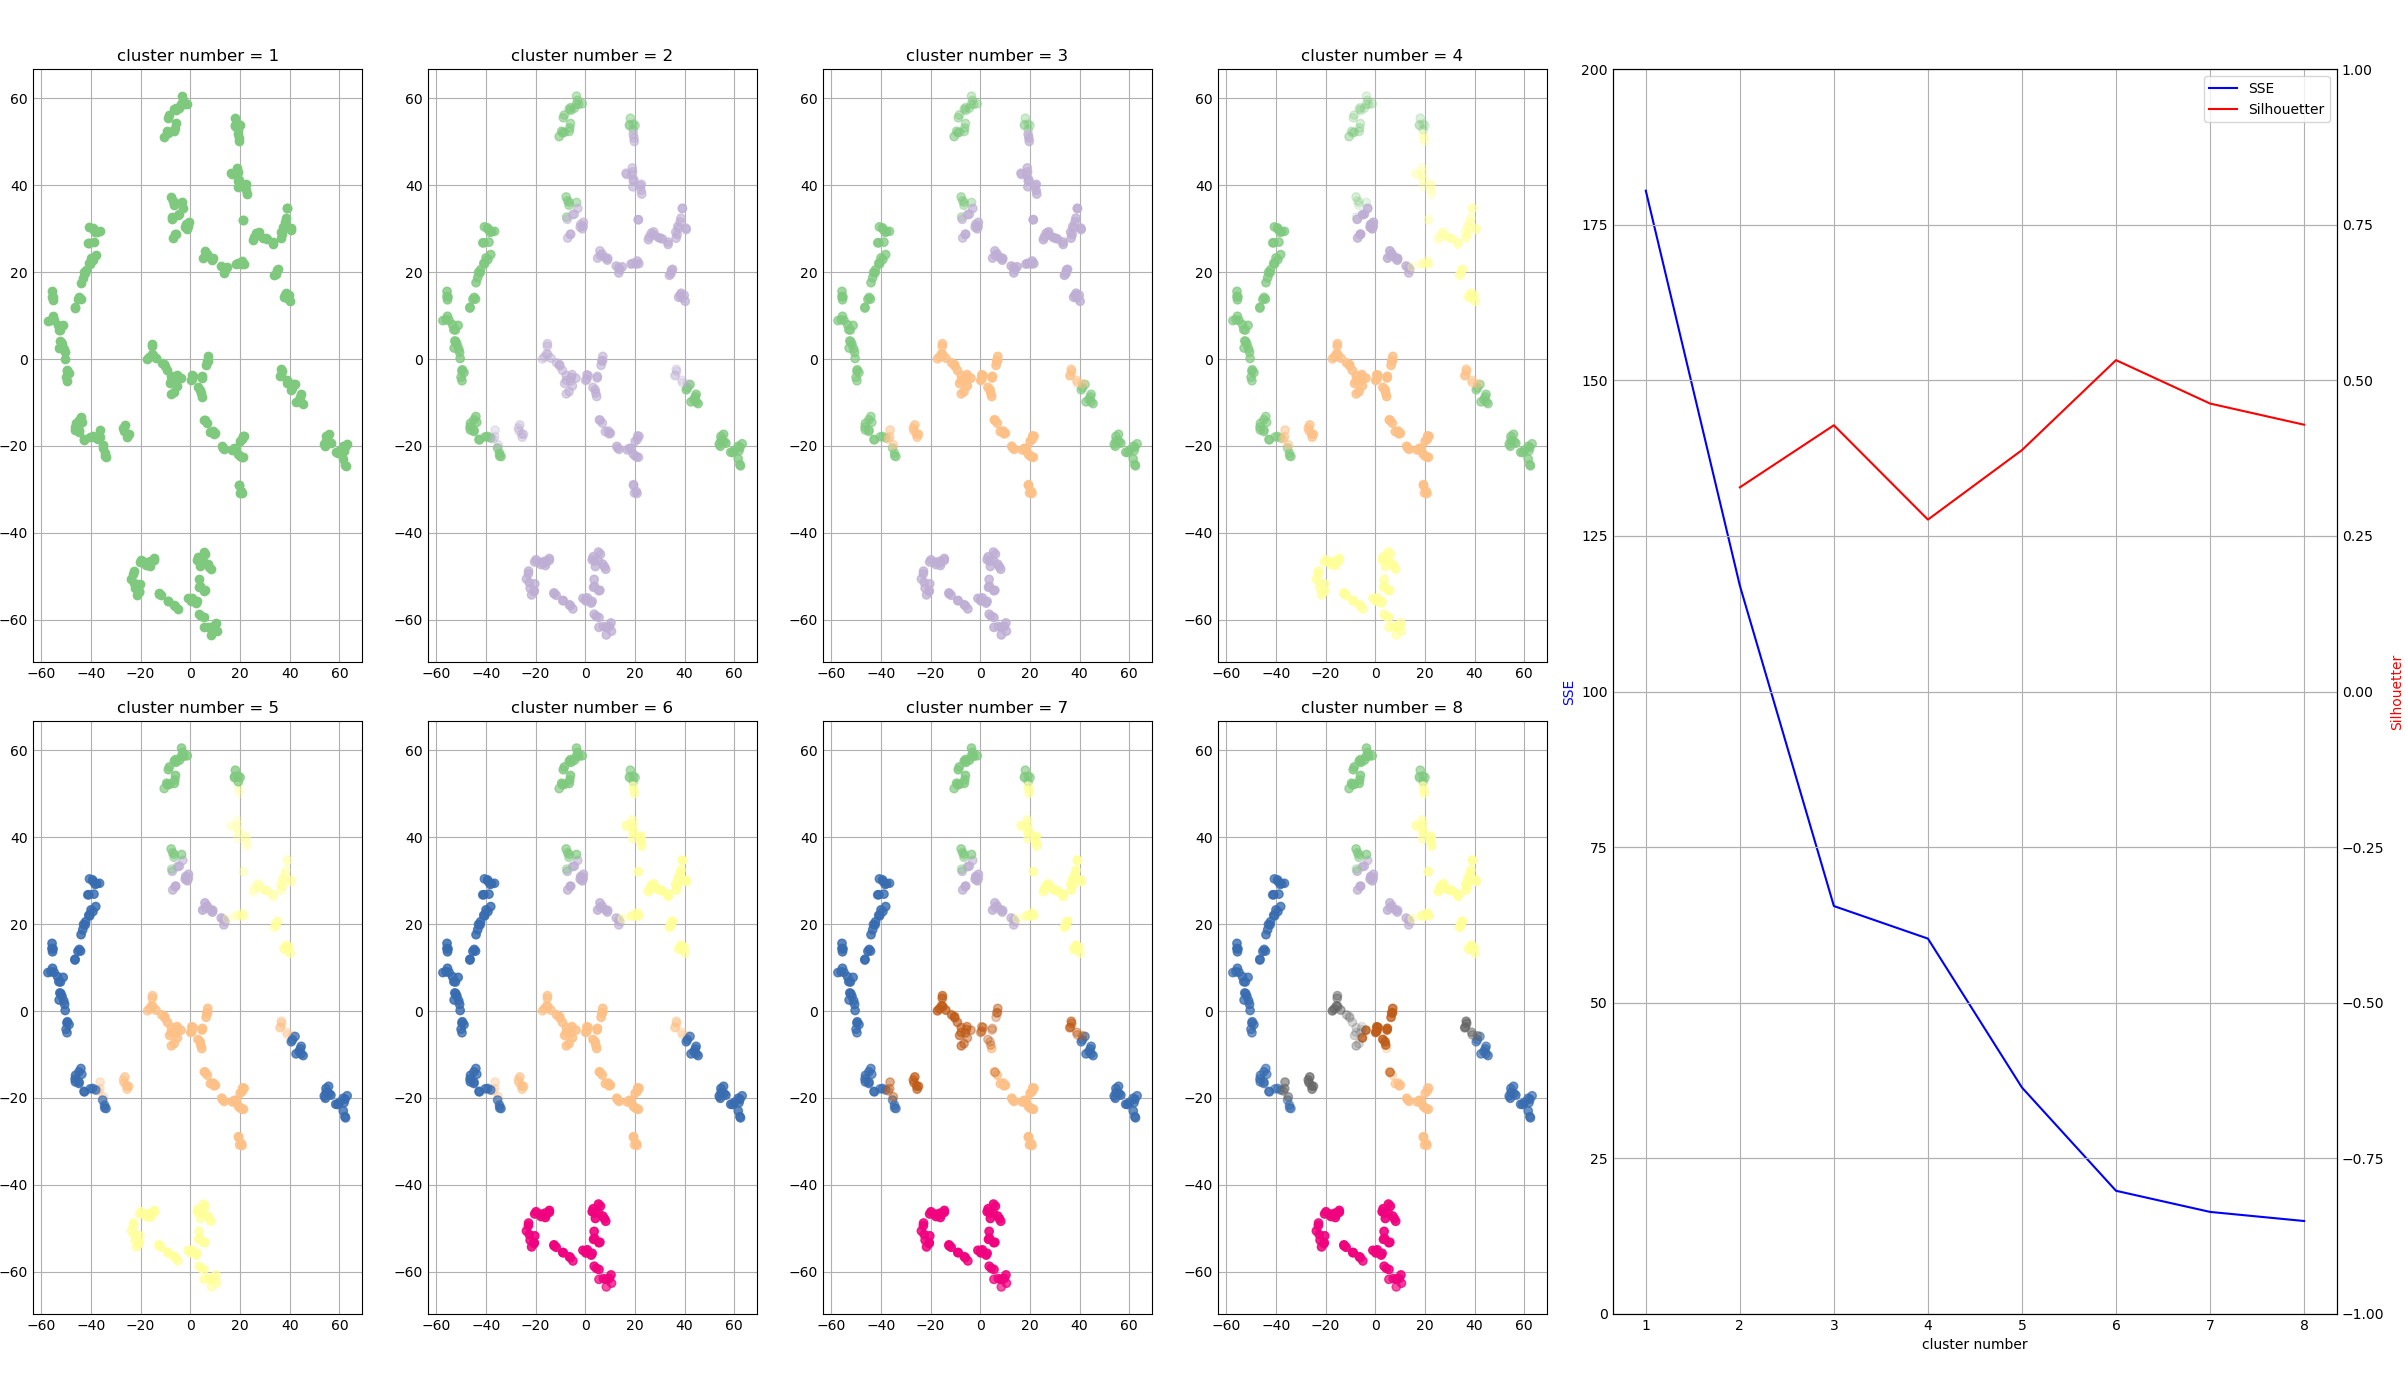
\includegraphics[scale=0.30]{Figure_1.png}
    \end{adjustbox}
    \caption{评价结果1}
\end{figure}
\begin{figure}[H]
    \begin{adjustbox}{center}
    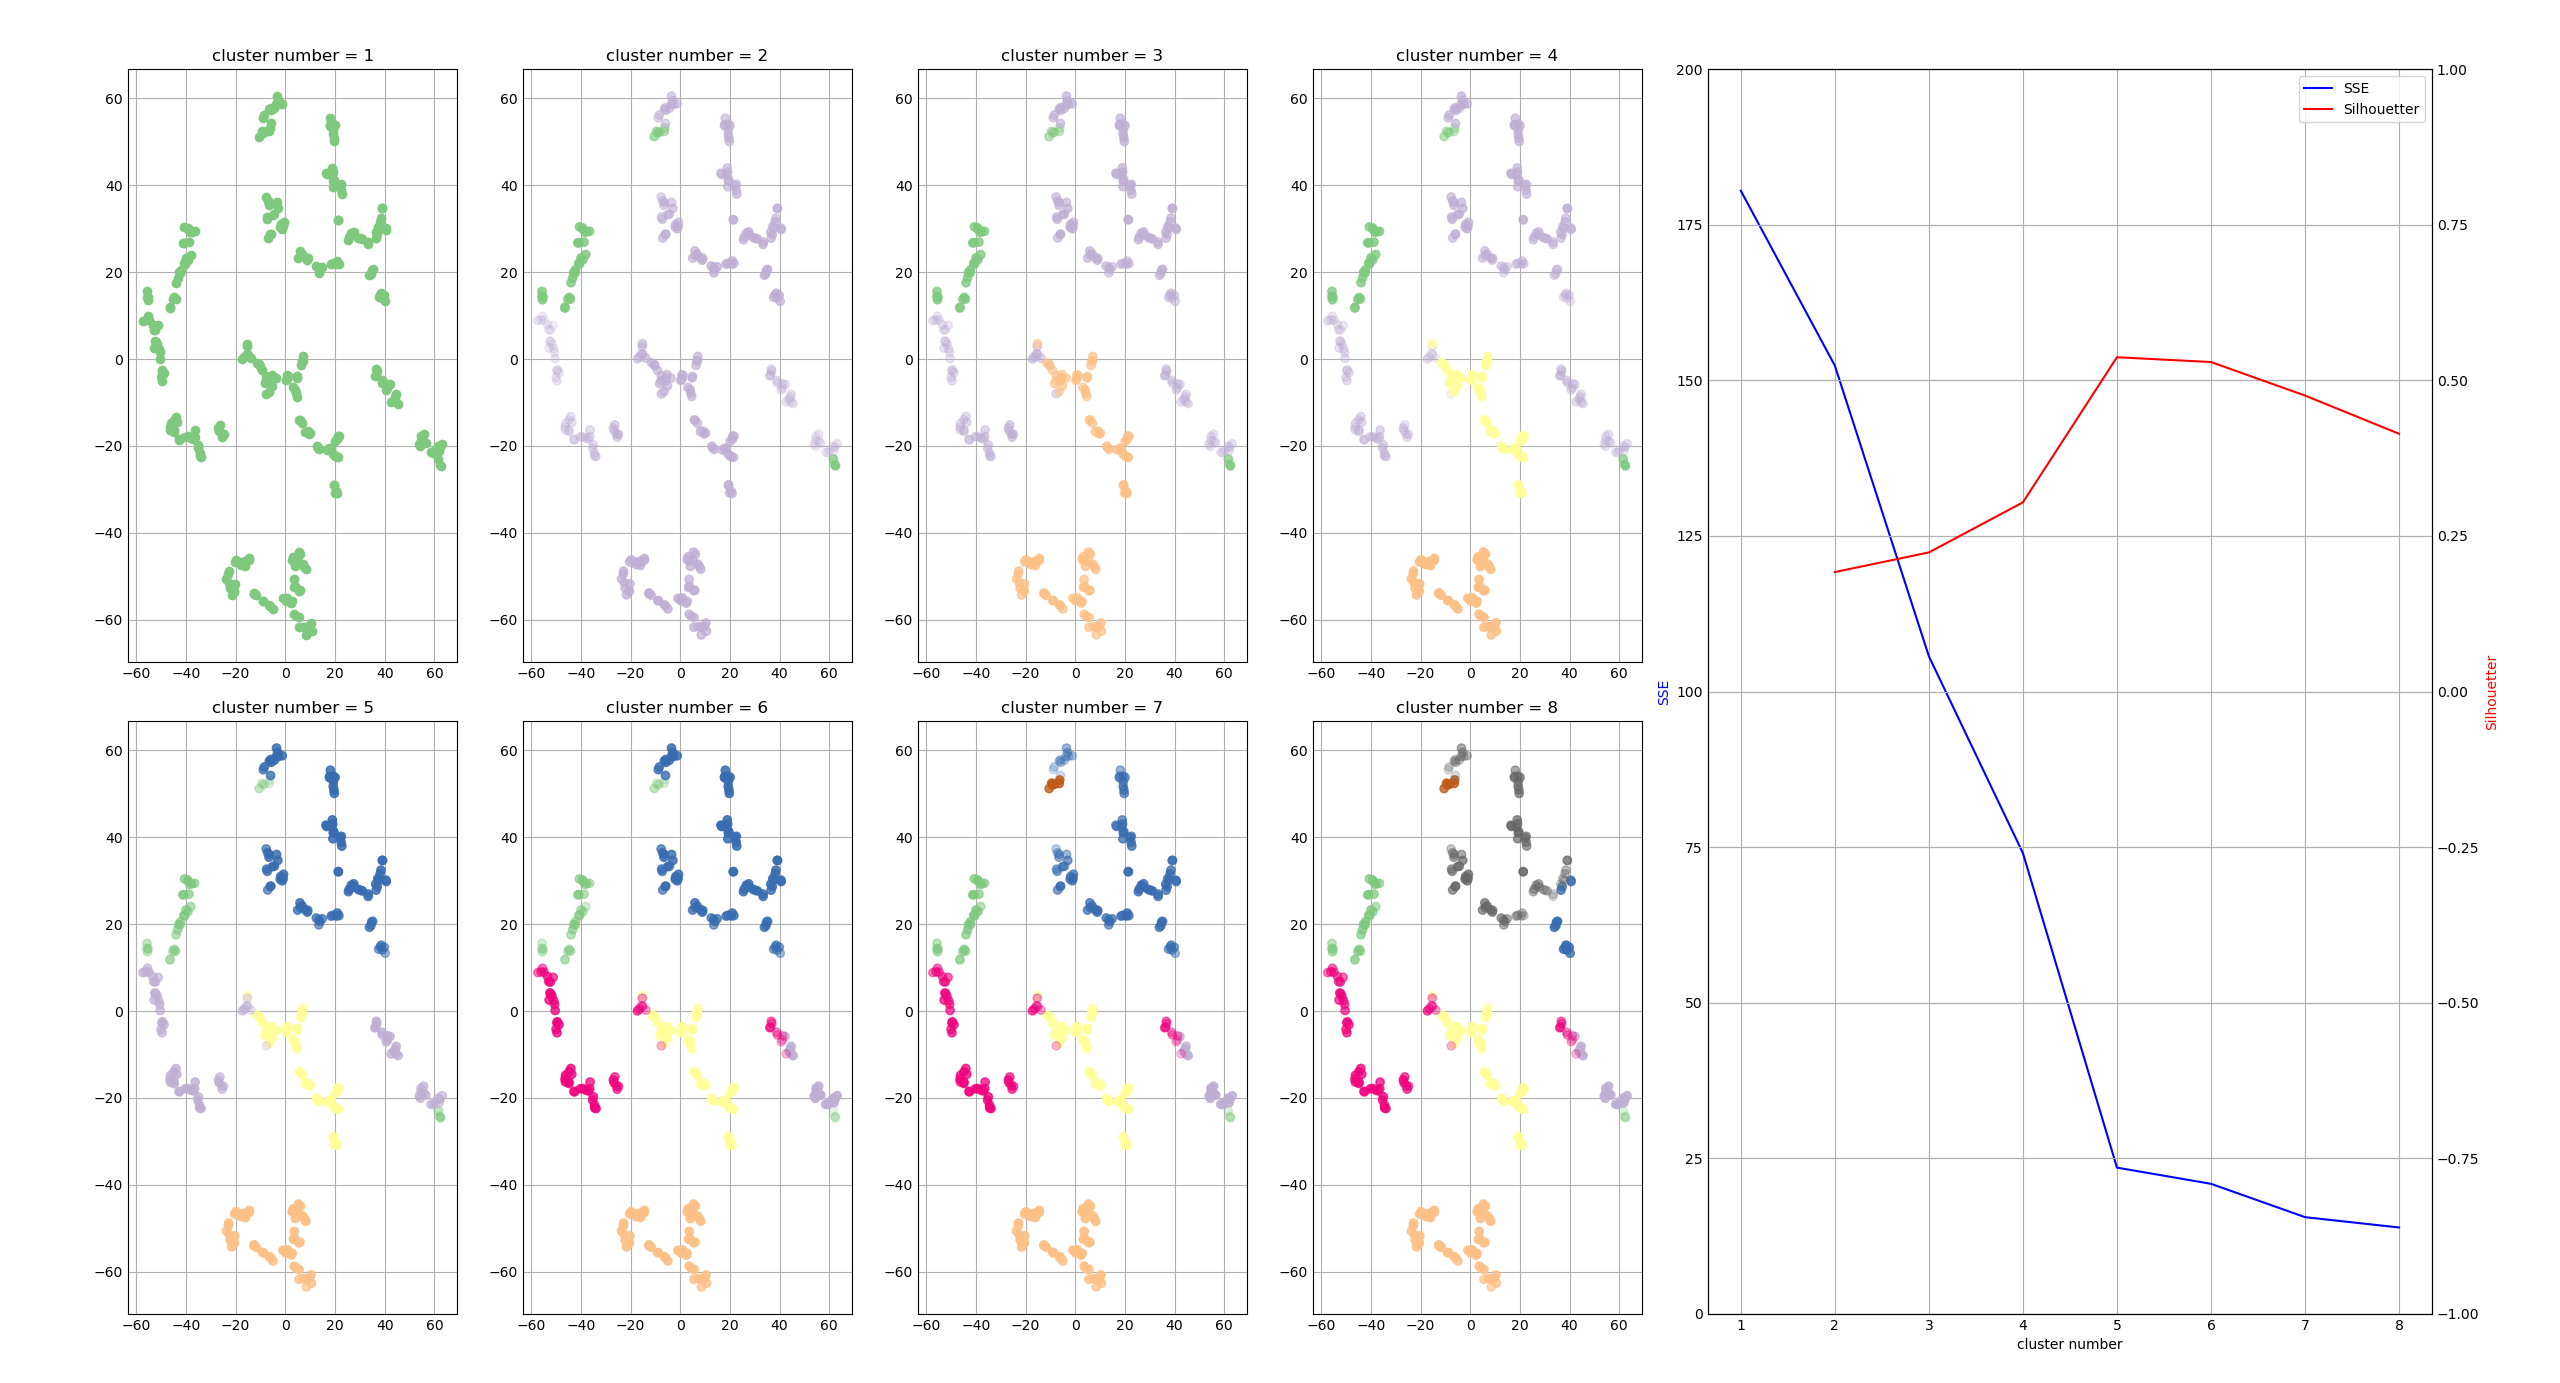
\includegraphics[scale=0.30]{Figure_2.png}
    \end{adjustbox}
    \caption{评价结果2}
\end{figure}
\begin{figure}[H]
    \begin{adjustbox}{center}
    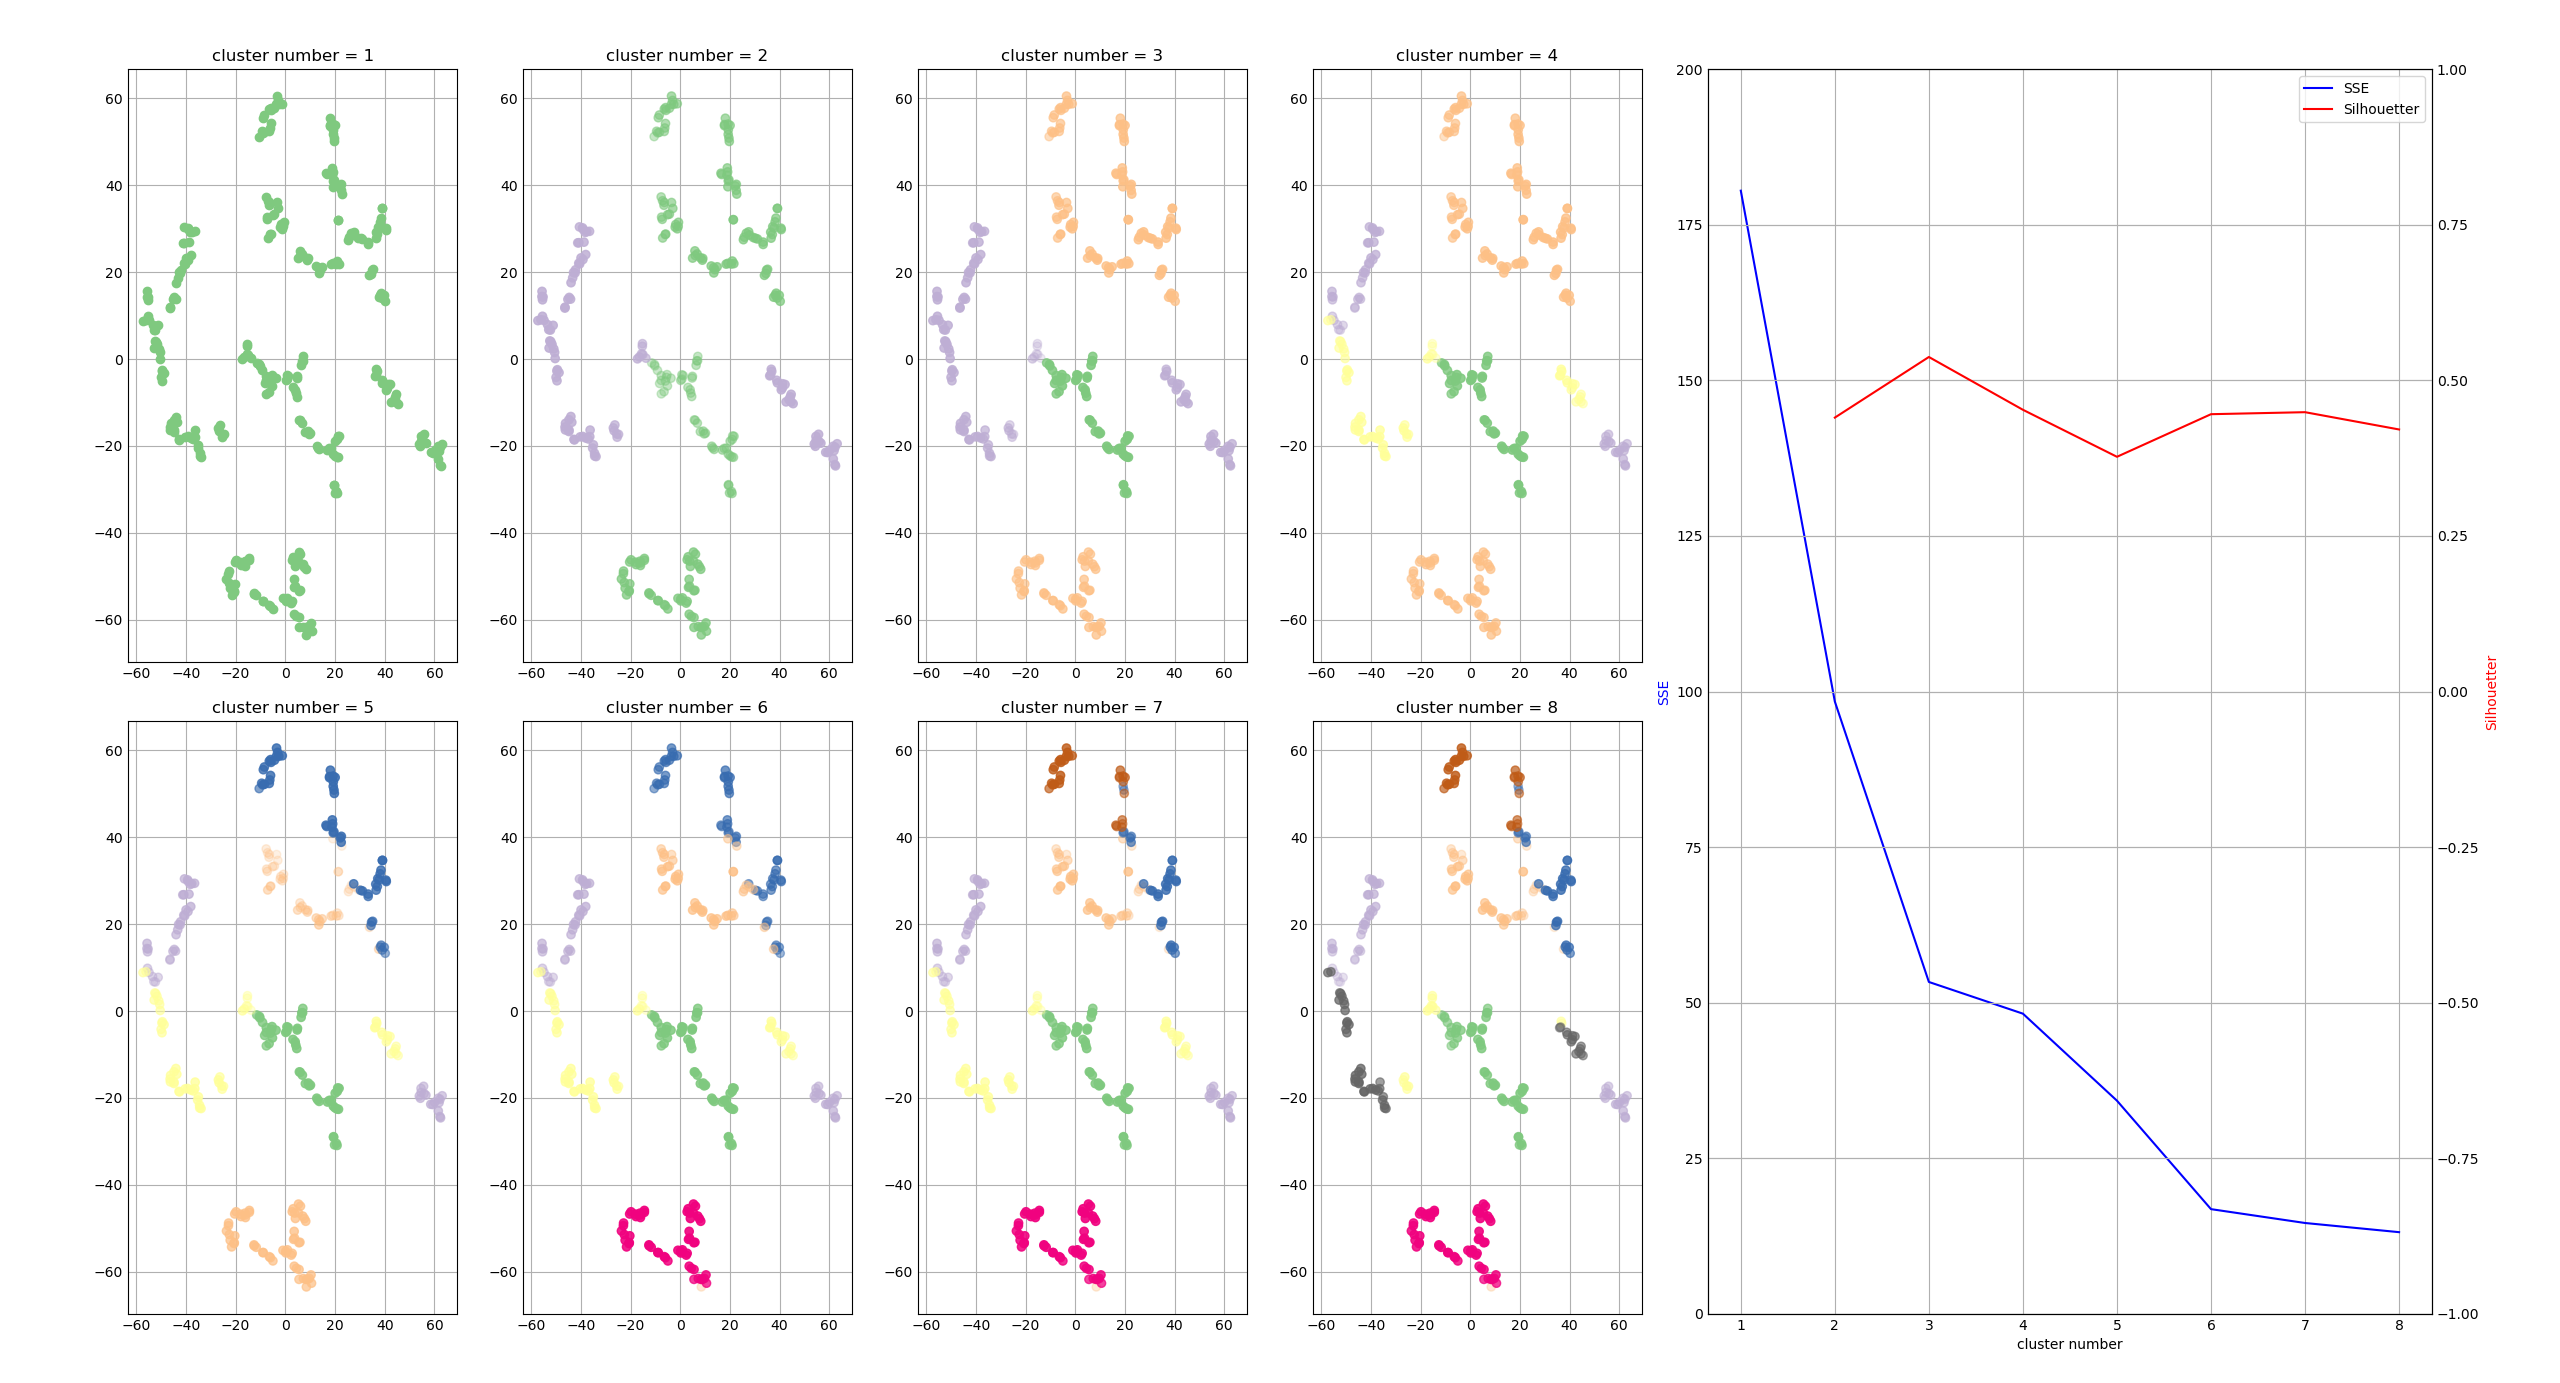
\includegraphics[scale=0.30]{Figure_3.png}
    \end{adjustbox}
    \caption{评价结果3}
\end{figure}
\section{改进之处}
本次实验中,我对常规的聚类可视化方法——散点图进行了改进。

许多数据集的维度都较高,为了能够利用散点图进行可视化,通常需要使用PCA或t-SNE等方法对数据进行降维。可是降维过后的数据往往丢失了
原来的相对位置关系,导致散点图中点之间的距离并不能反映出原来高维空间中的距离,从而难以直接根据散点图判断出数据点分类是否合理。
因此,我将各个数据点的轮廓系数映射到散点图对应点的透明度上,使得轮廓系数高的数据在散点图上显示清晰,表明该数据点的分类较为合理,
而轮廓系数低的数据在散点图上的醒目程度较低,表明对该数据点的分类并不可信。通过这一改进,散点图既可以通过颜色的不同来展现出高维数据的聚类结果,
同时还可以通过颜色的深浅来直观地反映出单个数据分类结果的好坏以及单个类簇的总体分类结果如何。
\section{心得体会}
本次实验过程中, Pandas以及Matplotlib库的使用大大简化了我的代码。以函数get\_sse为例,在使用DataFrame后,只需要一行代码便可以实现求均方和的功能,
这和上次使用C++实现ID3算法的体验有着极大差别,使我深刻体会到了掌握合适工具的重要性。

在算法评价的过程中,我也深刻地认识到了初始点的选取策略对于 K-Means算法的重要程度。通过优化初始点的选取策略, K-Means算法还有
很大的改进空间。

同时,在对于聚类结果进行可视化的过程中,我也感受到了可视化的重要性。如果没有进行可视化,聚类的结果只是一张张表格,从中很难直接获取有用的信息,
尤其是当数据量略大的时候。通过可视化,不仅仅能够将结果清晰直观地展现出来,还能够帮助人们从数据中发掘出更多有用的信息。
\end{document}